\documentclass[a4paper,12pt]{article}

\usepackage{fancyhdr}
\usepackage{lastpage}
\usepackage{amsmath}
\usepackage{tikz}
\usepackage{amsfonts}
\usepackage{csvsimple}
\usepackage{graphicx}


\newcommand{\V}[1]{\ensuremath{\vec{#1}}}
\newcommand{\F}[2]{\ensuremath{\frac{#1}{#2}}}
\newcommand{\Q}[1]{\newpage \section*{#1}}
\newcommand{\acc}[1]{\overset{..}{#1}}
\newcommand{\vel}[1]{\overset{.}{#1}}
\newcommand{\prt}[2]{\frac{\partial#1}{\partial#2}}
\newcommand{\LP}{\left(}
\newcommand{\RP}{\right)}

\pagestyle{fancy}
\lhead{Samuel Loomis}
\setlength{\headheight}{15pt}
\chead{Electromagnetism HW 3}
\rhead{\thepage\ of \pageref{LastPage}}
\lfoot{}
\cfoot{}
\rfoot{}

\begin{document}
\section{Problem 1}
Two dielectric materials ($\epsilon_1$ and $\epsilon_2$) meet at the infinitely big flat surface.  A free charge $q_f$ is placed some distance d away from the interface.  What is the electric field in each of the materials? (Hint: Use image charge method, but be careful about the boundary condition.)
\begin{figure}[h]
\centering
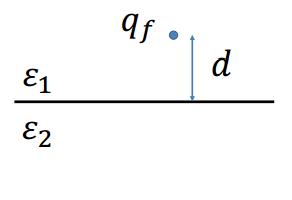
\includegraphics[width=2in]{dielectric_free_charge.png}
\end{figure}


\Q{Problem 2}
For a cricuit lying in a flat surgace, we define the associated magenetic momentum as \[\V{m}=IS\hat{n}\] where $I$ is the current, $S$ is the area and $\hat{n}$ is the surface normal from the right-hand rule.  For a more general circuit which could be winding in 3D space, the definition becomes the line integral \[\V{m}=\F{I}{2}\oint\V{r}\times d\V{l}\]

(I) Prove that both equations are equivalent when the circuit is confined to a flat surface. (II) Prove that the torque exerted on a current circuit by a uniform magnetic field is $\V{N}=\V{m}\times\V{B}$, even for a 3D circuit.

\Q{Problem 3}
Two spherical metal conductors have the same radius $a$ and are placed far apart at distance $d$. If they are both charged with total charge $Q$ and rotate along their own axis at angular speed $\omega$, what is the (approximate) ratio between their electric and magnetic interaction forces?

When a conductor is charged, the bits of charge spread out equally along the surface.  The surface charge density of these spheres are equal to the total charge divided by the surface area:
\[\sigma=\F{Q}{4\pi a^2}\]
The magnetic field generated by the sphere rotating can be found by considering the sphere as a bunch of rotating rings of charge.  Any point of charge at any $\theta$ and $\phi$ on the sphere is:
\[dq=\sigma*a^2sin(\theta)d\phi d\theta=\F{Q}{4\pi}sin(\theta)d\phi d\theta\]
While the sphere rotates at angular speed $\omega$, the velocity of and of these charges is equal to:
\[\V{v}=asin(\theta)\omega\hat{\phi}\]
and the current at any point is then
\[\V{I}=q\V{v}=\F{aQ\omega}{4\pi}sin^2(\theta)d\phi d\theta\hat{\phi}\]
The magnetic field at any point from this current is
\[\V{B}=\F{\mu_0}{4\pi}\int\F{\V{I}\times\hat{(r-r')}}{(r-r')^2}dl'\]
The force that a piece of one sphere feels from the other sphere magnetically will be
\[\V{F}_{mag}=I\int d\V{l}\times\V{B}\]
 where the magnetic field is from one shpere and the current as well as dl are from the sphere of interest.
\\
\\
Finding the magnetic field at any point on sphere 2 from sphere 1:
\begin{align*}
\V{B}_1=\F{\mu_0aQ\omega}{16\pi^2}\int\F{\hat{\phi_1}\times\hat{d}}{(d+r'_2-r'_1)^2}sin^2(\theta_1)d\phi_1d\theta_1
\end{align*}
\end{document}